\section{Konjunktur}
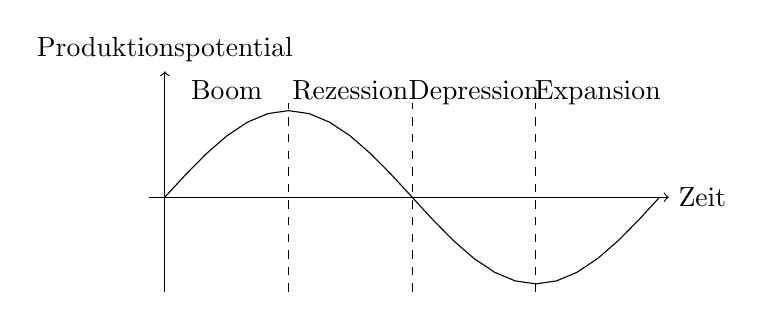
\begin{tikzpicture}[yscale=1]
	%\draw[very thin,color=gray] (-0.1,-1.1) grid (8.9,1.9);
	\draw[->] (-0.2,0) -- (6.4,0) node[right] {Zeit};
	\draw[->] (0,-1.2) -- (0,1.6) node[above] {Produktionspotential};
	\draw [domain=0:2*pi] plot (\x, {1.1 * (sin(\x r)});
	\draw[dashed] (pi/2, -1.2) -- (pi/2, 1.2);
	\draw[dashed] (pi, -1.2) -- (pi, 1.2);
	\draw[dashed] (3/2 * pi, -1.2) -- (3/2 * pi, 1.2);
	\draw (pi/4, 1.6) node [below] {Boom};
	\draw (3/4 * pi, 1.6) node [below] {Rezession};
	\draw (5/4 * pi, 1.6) node [below] {Depression};
	\draw (7/4 * pi, 1.6) node [below] {Expansion};
\end{tikzpicture}
\begin{description}\itemsep0em
	\item [Konjunktur] 
	Schwankung im Auslastungsgrad der Produktionsanlagen (der mittlere Auslastungsgrad liegt bei 85\%) -- Gemessen wird das reale BIP (d.\,h. um Preisänderungen korrigiertes nominelles BIP). Die Schwankungen lassen sich in Phasen unterteilen:
	
	\item [Boom] 
	(Hochkonjunktur) Auslastungsgrad nahe 100\%, Überstunden fallen an \dots
	\begin{itemize}\itemsep0em
		\item [$\Rightarrow$] Preiserhöhungen
		\item [$\Rightarrow$] mehr Investitionen
		\item [$\Rightarrow$] höhere Zinsen
	\end{itemize}
	Dies solange, bis der Markt überhitzt ist, und es zur nächsten Phase kommt:

	\item [Rezession]
	(Abschwung) Die Wirtschaft wächst oder schrumpft in zwei aufeinanderfolgenden Quartalen (d.\,h. sinkendes BIP). Die Auslastung geht zurück, liegt aber noch über dem Durchschnitt.

	\item [Depression]
	(Krise, \enquote{Tal der Tränen}) Das BIP ist um mindestens 10\% zurückgegangen oder das Negativ-Wachstum dauert mindestens 3 Jahre. Auf die Depression folgt die

	\item [Expansion]
	(Aufschwung) Die Wirtschaft wächst wieder.
	\begin{itemize}\itemsep0em
		\item [$\Rightarrow$] Konsumausgaben steigen
		\item [$\Rightarrow$] Investition steigen
	\end{itemize}
\end{description}
Es lässt sich freilich nur schwer abschätzen, in welcher Phase man sich zu einem beliebigen Zeitpunkt befindet. Es lässt sich jedoch folgende Faustregel anwenden:

\begin{center}
\begin{tabular}{|c|c|c|c|}
\cline{3-4}
\multicolumn{2}{c|}{} & \multicolumn{2}{c|}{\textbf{Lageeinschätzung}} \\ \cline{3-4}
\multicolumn{2}{c|}{} & \multicolumn{1}{c|}{\textbf{negativ}} & \multicolumn{1}{c|}{\textbf{positiv}} \\ \cline{1-4}
\multirow{2}{*}{\textbf{Erwartung}} &
\textbf{negativ} &
%% negative Erwartung, negative Lageeinschätzung
Depression & 
% negative Erwartung, positive Lageeinschätzung
Rezession \\ \cline{2-4}
	&
\textbf{hoch} & 
% positive Erwarung, negative Lageeinschätzung
Expansion & 
% positive Erwartung, positive Lageeinschätzung
Boom
\\ \cline{1-4}
\end{tabular}
\end{center}

\subsection{Konjunkturindikatoren}
\begin{description}\itemsep0em
	\item [Gleichlaufende] BIP, Investitionen in neue Maschinen, privater Konsum, Exporte und Umsätze
	\item [Nachhinkende] Preise, Arbeitslose, Löhne, Zinsen
	\item [Vorauseilende] Auftragseingänge, Geldmenge, Konsumentenstimmung, offene Baukredite (Einflüsse von aussen \enquote{exogene Schocks} sind allerdings nicht vorhersehbar)
\end{description}

Eine Branche ist mehr oder weniger stark von der Konjunktur abhängig. Je grösser die Einkommenselastizität eines Gutes, desto stärker der Einfluss der Konjunktur. (z.\,B. Luxusgüter werden in Krisen Zeiten weit weniger gekauft. Lebensmittel hingegen bleiben in etwa konstant).

\subsection{Ursachen für Schwankungen}
\begin{itemize}\itemsep0em
	\item Zinssenkung $\Rightarrow$ höhere Nachfrage $\Rightarrow$ höhere Preise\\
	(Nachfrage verschiebt sich nach rechts)
	\item Technologie $\Rightarrow$ geringe Produktionskosten $\Rightarrow$ tiefere Preise\\
	(Angebot verschiebt sich nach rechts)
	\item Naturkatastrophe $\Rightarrow$ Produktion schrumpft $\Rightarrow$ höhere Preise\\
	(Angebot verschiebt sich nach links)
	\item pessimistische Bevölkerung $\Rightarrow$ höhere Spareinlagen $\Rightarrow$ tiefere Preise\\
	(Nachfrage verschiebt sich nach links)
	\item Steuersenkungen $\Rightarrow$ Nachfrage und Angebot steigen (beide Kurven nach rechts)
\end{itemize}
 
\subsubsection{Einflussfaktoren auf die Konjunktur}
\begin{description}\itemsep0em
	\item [Nachfrageseitig] Private, staatliche und ausländische Nachfrage
	\item [Angebotsseitig] Verfügbarkeit an Realkapital, Arbeitern, Boden
	\item [Monetär] Geldmenge, Zinsen, Wechselkurse
	\item [Massenpsychologie] Hamsterkäufe
	\item [Ökologische Einflüsse] Katastrophen
	\item [Weltpolitische Situation] Aufstände, Kriege
	\item [Rahmenbedingungen] Steuern, Infrastruktur
\end{description}

Investitionen bewirken zweierlei:
\begin{itemize}\itemsep0em
	\item Kapazitätseffekt: Es kann mehr produziert werden (d.\,h. mehr Angebot)
	\item Einkommenseffekt: Das Volkseinkommen steigt (d.\,h. mehr Nachfrage)
\end{itemize}
Sind beide Effekt gleich gross, neutralisieren sie sich. Ansonsten führen sie zu:
\begin{itemize}\itemsep0em
	\item Kapazitätseffekt > Einkommenseffekt: Abschwung
	\item Einkommenseffekt > Kapazitätseffekt: Aufschwung
\end{itemize}

\subsection{Multiplikatortheorie}
Die \textbf{Grenzneigung zum Konsum} ($K$) bezeichnet den Anteil des Einkommens, der ausgegeben wird.
Der Multiplikator ($M$) ist:
\begin{equation*}
	M = \frac{1}{1 - K}
\end{equation*}
Ein investierter Betrag $i$ führt zu einem um $i \cot M$ erhöhten Gesamteinkommen,
weil zunächst $k\%$ wieder ausgegeben werden. Diese sind das Einkommen anderer, die davon wieder $k\%$ ausgeben usw.

$\Rightarrow$ Veränderungen in der Nachfrage wirken sich überproportional auf Einkommen und Beschäftigung aus.

\subsection{Akzeleratortheorie}
Veränderungen in der Nachfrage lösen überpropertionale Änderungen der Investionen aus.

Erhöht sich die Nachfrage und sind neue Maschinen notwendig, so müssen 
\begin{enumerate}\itemsep0em
	\item Ersatzinvestitionen für die alten Maschinen getätigt werden
	\item neue Maschinen angeschafft werden
\end{enumerate}
Geht die Nachfrage zurück, so müssen trotzdem Ersatzinvestitionen stattfinden

\subsection{Zins-Fallen}
\begin{description}\itemsep0em
	\item [Liquiditätsfalle] 
	Situation einer Volkswirtschaft, in der die offiziellen Zinssätze so weit gegen null gefallen sind, dass die herkömmliche Geldpolitik versagt. Das Phänomen, dass Geld bei sinkenden Zinssätzen nicht mehr für Investitionen angeboten wird und somit dem Wirtschaftskreislauf tendenziell entzogen wird, weil man auf bessere Investionsmöglichkeiten wartet.

	\item [Investitionsfalle] beschreibt das ökonomische Phänomen, dass Unternehmen in Zeiten einer Depression selbst dann nicht investieren, wenn die Zinsen sehr niedrig sind. Ursächlich hierfür ist, dass die Unternehmen nicht einmal die bereits vorhandenen Produktionskapazitäten auslasten; dennoch weiter zu investieren wäre also widersinnig.
	
\end{description}
